%
% This is a borrowed LaTeX template file for lecture notes for CS267,
% Applications of Parallel Computing, UCBerkeley EECS Department.
% Now being used for CMU's 10725 Fall 2012 Optimization course
% taught by Geoff Gordon and Ryan Tibshirani.  When preparing
% LaTeX notes for this class, please use this template.
%
% To familiarize yourself with this template, the body contains
% some examples of its use.  Look them over.  Then you can
% run LaTeX on this file.  After you have LaTeXed this file then
% you can look over the result either by printing it out with
% dvips or using xdvi. "pdflatex template.tex" should also work.
%

\documentclass[twoside]{article}
\setlength{\oddsidemargin}{0.25 in}
\setlength{\evensidemargin}{-0.25 in}
\setlength{\topmargin}{-0.6 in}
\setlength{\textwidth}{6.5 in}
\setlength{\textheight}{8.5 in}
\setlength{\headsep}{0.75 in}
\setlength{\parindent}{0 in}
\setlength{\parskip}{0.1 in}

%
% ADD PACKAGES here:
%

\usepackage{amsmath,amsfonts,graphicx}
\graphicspath{ {./images/} }

%
% The following commands set up the lecnum (lecture number)
% counter and make various numbering schemes work relative
% to the lecture number.
%
\newcounter{lecnum}
\renewcommand{\thepage}{\thelecnum-\arabic{page}}
\renewcommand{\thesection}{\thelecnum.\arabic{section}}
\renewcommand{\theequation}{\thelecnum.\arabic{equation}}
\renewcommand{\thefigure}{\thelecnum.\arabic{figure}}
\renewcommand{\thetable}{\thelecnum.\arabic{table}}

%
% The following macro is used to generate the header.
%
\newcommand{\lecture}[4]{
    \pagestyle{myheadings}
    \thispagestyle{plain}
    \newpage
    \setcounter{lecnum}{#1}
    \setcounter{page}{1}
    \noindent
    \begin{center}
    \framebox{
        \vbox{\vspace{2mm}
    \hbox to 6.28in { {\bf CPSC 421: Introduction to Theory of Computing
    \hfill Winter Term 1 2018-19} }
        \vspace{4mm}
        \hbox to 6.28in { {\Large \hfill Lecture #1: #2  \hfill} }
        \vspace{2mm}
        \hbox to 6.28in { {\it Lecturer: #3 \hfill Scribes: #4} }
        \vspace{2mm}}
    }
    \end{center}
    \markboth{Lecture #1: #2}{Lecture #1: #2}

%    {\bf Note}: {\it LaTeX template courtesy of UC Berkeley EECS dept.}
%
%    {\bf Disclaimer}: {\it These notes have not been subjected to the
%    usual scrutiny reserved for formal publications.  They may be distributed
%    outside this class only with the permission of the Instructor.}
%    \vspace*{4mm}
}
%
% Convention for citations is authors' initials followed by the year.
% For example, to cite a paper by Leighton and Maggs you would type
% \cite{LM89}, and to cite a paper by Strassen you would type \cite{S69}.
% (To avoid bibliography problems, for now we redefine the \cite command.)
% Also commands that create a suitable format for the reference list.
\renewcommand{\cite}[1]{[#1]}
\def\beginrefs{\begin{list}%
        {[\arabic{equation}]}{\usecounter{equation}
            \setlength{\leftmargin}{2.0truecm}\setlength{\labelsep}{0.4truecm}%
            \setlength{\labelwidth}{1.6truecm}}}
\def\endrefs{\end{list}}
\def\bibentry#1{\item[\hbox{[#1]}]}

%Use this command for a figure; it puts a figure in wherever you want it.
%usage: \fig{NUMBER}{SPACE-IN-INCHES}{CAPTION}
\newcommand{\fig}[3]{
            \vspace{#2}
            \begin{center}
            Figure \thelecnum.#1:~#3
            \end{center}
    }
% Use these for theorems, lemmas, proofs, etc.
\newtheorem{theorem}{Theorem}[lecnum]
\newtheorem{lemma}[theorem]{Lemma}
\newtheorem{proposition}[theorem]{Proposition}
\newtheorem{claim}[theorem]{Claim}
\newtheorem{corollary}[theorem]{Corollary}
\newtheorem{definition}[theorem]{Definition}
\newenvironment{proof}{{\bf Proof:}}{\hfill\rule{2mm}{2mm}}

% **** IF YOU WANT TO DEFINE ADDITIONAL MACROS FOR YOURSELF, PUT THEM HERE:

\newcommand\E{\mathbb{E}}

\begin{document}
%FILL IN THE RIGHT INFO.
%\lecture{**LECTURE-NUMBER**}{**DATE**}{**LECTURER**}{**SCRIBE**}
\lecture{6}{September 17}{Nicholas Harvey}{Kaitian Xie}
%\footnotetext{These notes are partially based on those of Nigel Mansell.}

\section{Danger with Intuition}

$L =\{w: w \text{ has a equal \# of occurrences of substrings 01 and 10 }\}$ 

This \underline{is} a regular, surprisingly (Ex 1.48).

\begin{figure*}[ht]
  \centering
  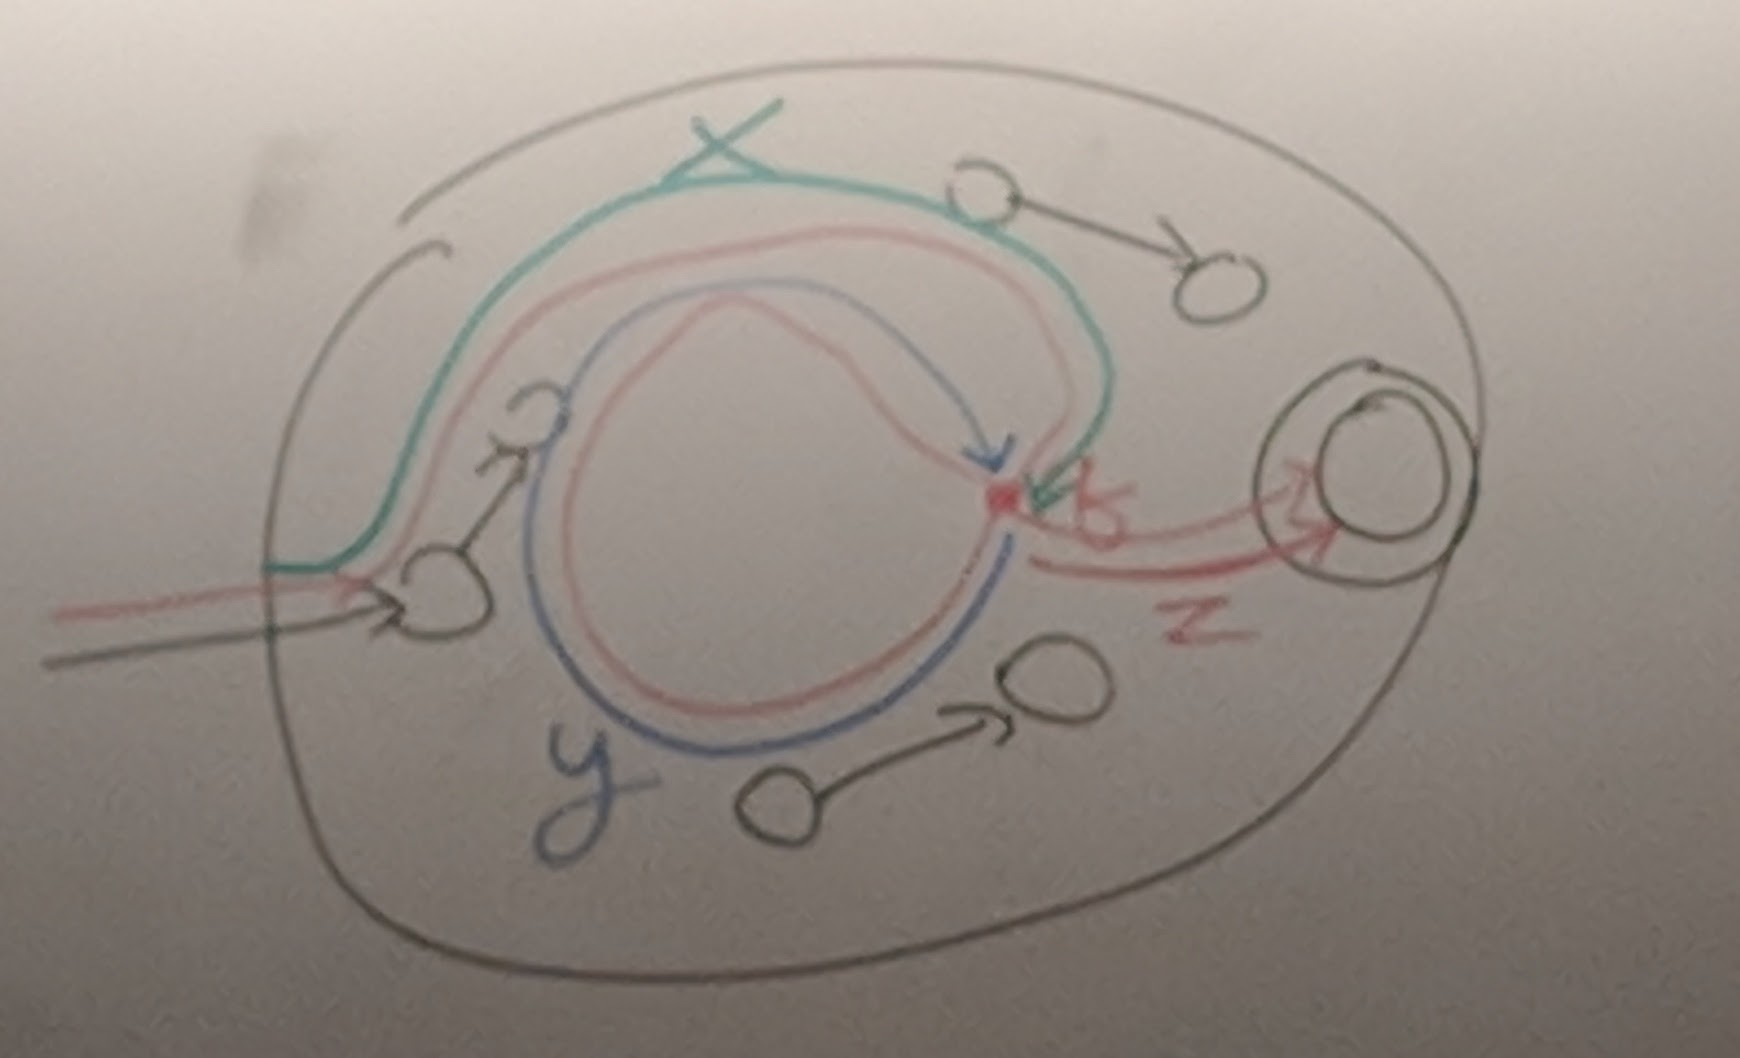
\includegraphics[scale=0.2]{img1}
\end{figure*}

Give the DFA a long input string $w$. \underline{Computation path on input $w$} must contain a cycle. Let $x$ be the part of input that was processed before arriving at $q$. While going round cycle, read $y$ from input. After cycle, we read $z$ from input.

What if input were $xyyz$. The DFA also accepts; we just travel cycle twice.

\underline{Message}: If $L$ is regular, then for a sufficiently long string $w \in L$, we can repeat its special substring $y$, to get another string in $L$.

\underline{Refinement of Message}: Let $p$ = \# states of DFA. If $|w| \geq p$ then computation path has length $\geq p + 1$. By Pigeonhole Principle, a cycle exists. So we can assume $|xy| \leq p$. That's enough to get a cycle.

\underline{Important Point}:
\begin{itemize}
  \item We can (usually) use Pumping Lemma to prove that a language is not regular by proving that it satisfies the negation of Pumping Condition.
  \item We \underline{cannot} use P.L to prove that a language is regular.
\end{itemize}

How to negate a statement with logical quantifiers:
\begin{itemize}
  \item $\exists x$ s.t. $f$ becomes $\forall x$, NOT $f$
  \item $\forall x$, $g$ becomes $\exists x$ s.t. NOT $g$
\end{itemize}

\end{document}
